\documentclass{beamer}

\usepackage{listings}
\usepackage{color}

\definecolor{dkgreen}{rgb}{0,0.6,0}
\definecolor{gray}{rgb}{0.5,0.5,0.5}
\definecolor{mauve}{rgb}{0.58,0,0.82}

\lstset{frame=tb,
  language=Haskell,
  aboveskip=3mm,
  belowskip=3mm,
  showstringspaces=false,
  columns=flexible,
  basicstyle={\small\ttfamily},
  numbers=none,
  numberstyle=\tiny\color{gray},
  keywordstyle=\color{blue},
  commentstyle=\color{dkgreen},
  stringstyle=\color{mauve},
  breaklines=true,
  breakatwhitespace=true,
  tabsize=3
}

\usepackage{amsmath}
\usepackage{amssymb}
\usepackage{tikz}

\usetheme{CambridgeUS}
\setbeamertemplate{caption}[numbered]


\AtBeginSection[]{
\begin{frame}
	\vfill
	\centering
	\begin{beamercolorbox}[sep=8pt,center,rounded=true,shadow=true]{title}
	  {\usebeamerfont{title}\insertsectionhead}\par%
	\end{beamercolorbox}
	\vfill
\end{frame}
}
  

\title{FP Project Presentation: Iris NN Inference}
\author{Santripta Sharma}
\date{\today}

\begin{document}

\begin{frame}
	\titlepage
\end{frame}	

\section{Problem Definition \& Solution Specification}

\begin{frame}{Problem Statement \& Requirements}
  \begin{block}<1->{Problem Statement}
    Develop a classification model over the Iris Dataset and store the model. Then write a Haskell code to restore the model, input new data (based on the four features of the iris) and generate a prediction in real time.
    \begin{enumerate}
      \item<2-> Input: The Iris Dataset.
      \item<2-> Output: Real-time prediction for the class of the flower of a new data row containing the sepal width, petal width, sepal length and petal length.
      \item<3-> Method: You can use Python to train and save a classification model (SVM or NN). However, restoring the model and the real-time prediction of a new data row has to be written only in Haskell.
    \end{enumerate}
  \end{block}
\end{frame}

\begin{frame}{Problem Statement \& Requirements}
  From this statement, we derive our requirements:
  \begin{block}{Requirements}
    \begin{itemize}
      \item<2-> The system should be able to load a trained classification model.
      \item<3-> Given any new data point of the same format as the iris dataset by the user, the system should be able to use the loaded model to make a prediction on this data and report it to the user.
      \item<4-> The inference part of the system should be as performant as possible.
    \end{itemize}
  \end{block}
\end{frame}

\begin{frame}{Specifications}
  In order to meet these requirements, we build a system with the following feature set:
  \begin{enumerate}
    \item<2-> Parsing capabilities to restore the shape, weights, and biases of \textbf{an arbitrary} FFN-based classifier from a file.
    \item<3-> Interactive \& batched modes of performing inference. \begin{itemize}
      \item \textbf{Interactive}: The user enters a single new datapoint and gets predictions for it in real-time. Structured as a Read-Eval-Print-Loop (REPL).
      \item<4-> \textbf{Batched}: The user provides many datapoints in a csv file, and receives predictions for each point. Additionally, the system reports aggregate statistics.
    \end{itemize}
  \end{enumerate}  
\end{frame}

\section{System Design \& Architecture}
\begin{frame}{High-level view}
  \begin{figure}
    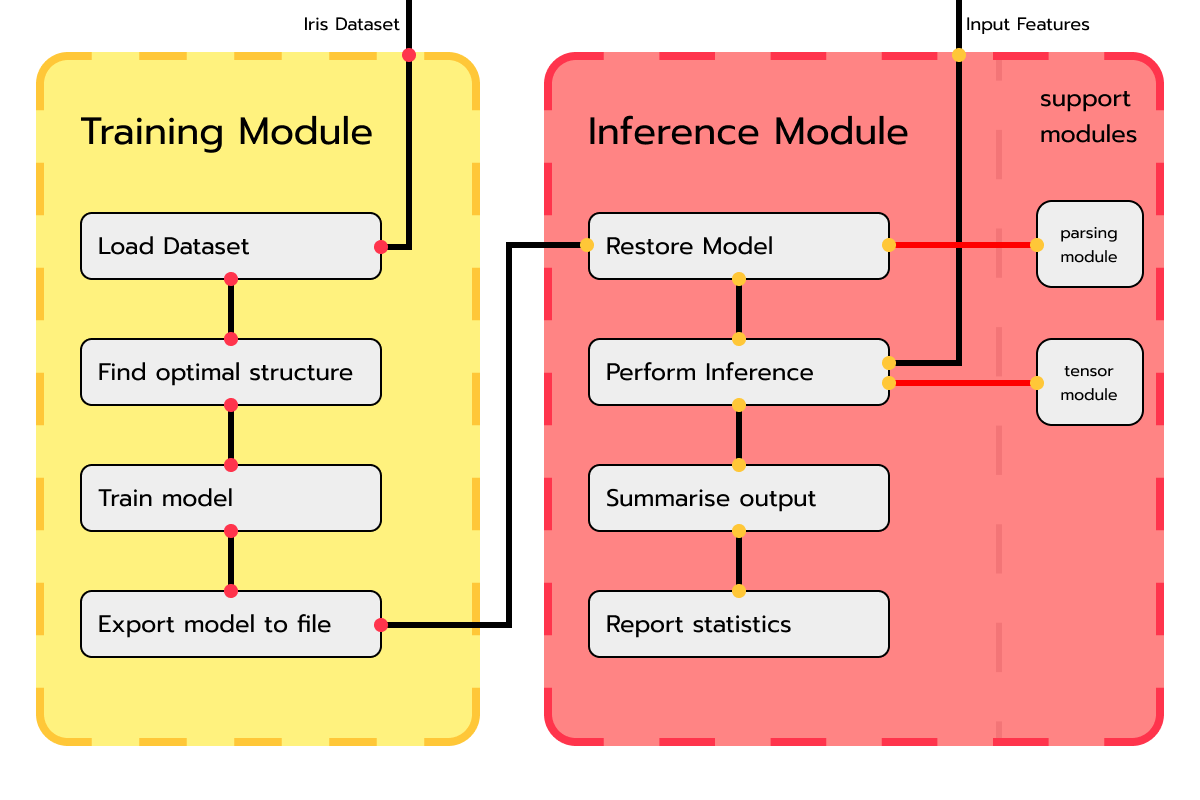
\includegraphics[width=0.95\textwidth]{../images/modules.png}
  \end{figure}
  \only<2>{%
  \tikz[overlay,remember picture]
  \node[fill=blue,text=white,rotate=90] at ([xshift=-0.8cm,yshift=-0.9cm]current page.center){what's happening here?};
  }
\end{frame}

\begin{frame}[fragile]{Model File Format}
  \begin{itemize}
    \item For the prototyping stage, we opt to use a plaintext format for the trained model parameters, since this allows easier debugging and editing.
    \item<2-> Using the propagation formula $Wx + b$, we can infer the incoming and outgoing dimension of each layer from its weights and biases matrices alone.
  \end{itemize}
  \pause
  \pause
  Then, our model file format can be described using this output spec:
  \begin{verbatim}
    for each layer in the network:
    weights matrix
    biases vector
  \end{verbatim}
  \vspace*{-16pt}
  If we make the assumption that the network uses a ReLU activation at every layer except the last, where softmax is used, this information is sufficient to restore the network.
\end{frame}

\begin{frame}
  \frametitle{Training Module}

  \begin{itemize}
    \item The training module provides us with a set of models we can use to test our inference module.
    \item<2-> Using a 5-fold cross-validation, we perform a grid search to find the best 5 network shapes for the architecture mentioned above, as well as the worst shape.
    \item<3-> We then train these 6 models on a split of the dataset, and save them to disk.
  \end{itemize}

\end{frame}

\begin{frame}[fragile]
  \frametitle{Inference Module}

  \begin{itemize}
    \item The inference module produces an executable with the following signature: \verb|inference-exe <path_to_model_file> [<path_to_batch_csv>]|
    If the second, optional argument is omitted, it starts in interactive mode. Otherwise, it starts in batched mode.
    \item<2-> It first restores the model from the given model file. Here, we utilise the parsing support module.
    \item<3-> Through this parsing process, the model shape, and its parameters are loaded into a data structure which takes the form of a list of layers.
    \item<4-> Then, based on which mode it was started in, it collects user input accordingly, and uses the tensor support module to perform the inference, and reports the prediction \& activation probabilities to the user.
  \end{itemize}

\end{frame}

\begin{frame}
  \frametitle{Example}
  \begin{figure}
    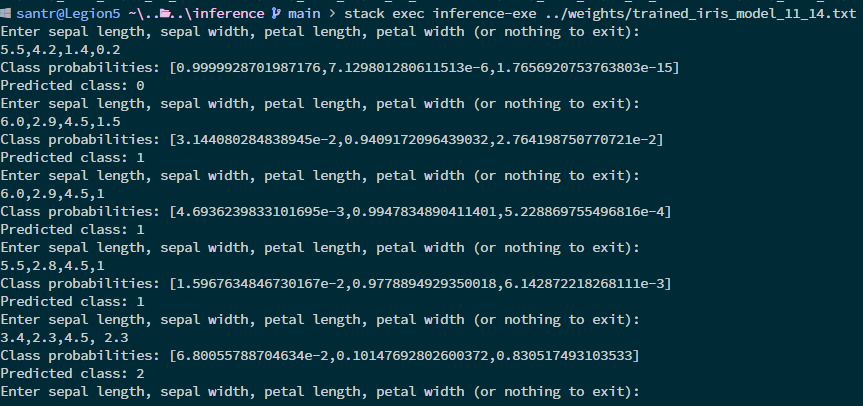
\includegraphics[width=0.9\textwidth]{../images/examples.png}
    \caption{examples of inference in interactive mode}
  \end{figure}
\end{frame}

\section{Tooling}

\begin{frame}
  \frametitle{Languages}

  \textbf{Training Module}\\
  The training module is written in \textbf{python}, using \textbf{numpy}, \textbf{pandas}, and \textbf{sklearn} to perform the data processing \& model training/selection.\bigskip

  \textbf{Inference Module}\\
  The inference module is written in \textbf{Haskell}. We use the \textbf{Haskell Tool Stack} (or just Stack) as our build tool.\bigskip

  \textbf{Misc/Testing}\\
  A mix of bash \& python scripts is used to implement the end-to-end tests and certain convenience utilities.
\end{frame}

\begin{frame}
  \frametitle{Inference Module Dependencies}

  \begin{itemize}
    \item \textbf{matrix \& vector}\\
    \onslide<2->{As the name suggests, these two packages provide a Matrix \& Vector type respectively, also providing the definitions for common mathematical operations on them.\bigskip}

    \onslide<3->{Together, they form the tensor support module, which is used to finally perform the inference once the inputs have been parsed.}

    \item<4-> \textbf{parsec}\\
    Parsec is Haskell's standard parser combinator library, allowing us to write atomic parsers and compose them together. Parsec forms the foundations of the parsing support module, which is used for parsing both the model files \& csv files for batched input mode.\bigskip

    \onslide<5->{Discussion of the specifics of the parser implementations is deferred to the Prototype Details section.}
  \end{itemize}

\end{frame}

\section{Test Plan}

\begin{frame}
  \frametitle{Strategy}
  
  The plan is to implement a test suite consisting of both unit \& end-to-end tests. Additionally, we will be profiling our code to ensure it meets the real-time requirements.\bigskip

  Unit tests will be implemented using \textbf{HSpec}, the testing framework provided by \textbf{Stack}.
\end{frame}

\begin{frame}
  \frametitle{Unit Testing}

  First, we note that the training module does not require testing, due to its simplicity and it almost exclusively using sklearn library functions.\medskip
  
  \onslide<2->{For the inference module, all the parser functions, and many of the inference functions are complex enough to warrant unit testing.\medskip}

  \onslide<3->{In order to cover the large space of inputs for these functions, we plan to heavily depend on generated test suites, as opposed to hand-crafted ones.\medskip}

  \onslide<4->{Consider two examples:
  \begin{itemize}
    \item \textbf{For the matrix parser:} We generate random real-valued matrices, stringify them, run them through the parser, and verify that the same matrix is recovered.
    \item \textbf{For batch softmax:} Use single-vector inference softmax as oracle and verify batch softmax on generated output activation matrices.
  \end{itemize}}
\end{frame}

\begin{frame}
  \frametitle{E2E Testing}

  We use an end-to-end test to verify the correctness of our inference module. Here, we treat our sklearn model as an oracle, randomly generating many batches of feature vectors (in addition to the existing test split), running them through both our oracle \& the inference module, and comparing the output activations.

\end{frame}

\section{Prototype Details}

\begin{frame}
  \frametitle{Feature Set}

  The prototype implements the following features:
  \begin{itemize}
    \item Complete restoration of any feed-forward classifier, given its parameters in the model file format, assuming it uses ReLU + Softmax activations.
    \item Interactive mode REPL, where the user can enter new datapoints, and get prediction outputs (activations + class label) for them.
    \item Batch mode, where the user can provide a csv file of datapoints to run inference on, and get prediction outputs for each point.
  \end{itemize}
\end{frame}

\begin{frame}
  \frametitle{Limitations of the Prototype}

  \begin{itemize}
    \item Lack of runtime checks for user input, leading to a restrictive input format \& several non-graceful exits, without any useful feedback to the user.
    \item Class of models that works limited to ReLU + Softmax activation based classifiers (large but not comprehensive).
    \item The csv input in batch mode can't end on a blank line (parser bug).
    \item Batch mode doesn't provide summary statistics.
  \end{itemize}

\end{frame}

\section {Selected Functionality}

\begin{frame}
  \frametitle{Overview}

  We will discuss the implementation details of two key components of the system, the parsing support module \& inference module, by looking at examples of haskell code, how they fit together, and how they evolve.\bigskip

  \pause

  For this, we will look at two examples - parsing of model files using parser combinators, and the pitfall of initially specialising the inference functions to single vectors.

\end{frame}

\begin{frame}[fragile]
  \frametitle{Parsing Model Files - Numbers}

  \begin{lstlisting}
    number :: Parser Double
    number = do
      sign <- option "" $ string "-"
      int <- many1 digit <?> "integer part"
      dec <- option "" $ do
        void $ char '.'
        frac <- many1 digit
        return $ '.' : frac
      pow <- option "" $ do
        void $ char 'e'
        esign <- option "" $ string "-" <|> string "+"
        num <- many1 digit
        let epart = 'e':(esign ++ num)
        return epart
      let num = read (sign ++ int ++ dec ++ pow) :: Double
      return num	
  \end{lstlisting}

\end{frame}

\begin{frame}[fragile]
  \frametitle{Parsing Model Files - Vectors}

  \begin{lstlisting}
    vector :: Parser [Double]
    vector = do
      void $ char '['
      eatWhitespace
      numbers <- sepEndBy number (many1 whitespace)
      void (char ']' <?> "vector closing bracket")
      return numbers
  \end{lstlisting}
    
\end{frame}

\begin{frame}[fragile]
  \frametitle{Parsing Model Files - Matrices}

  \begin{lstlisting}
    matrix :: Parser (Matrix Double, Int, Int)
    matrix = do
      void $ char '['
      eatWhitespace
      rows <- sepEndBy vector (many1 whitespace)
      void (char ']' <?> "matrix closing bracket")
      let nRows = length rows
      let nCols = length $ head rows
      return (Mat.fromList nRows nCols (concat rows), nRows, nCols)
  \end{lstlisting}
    
  And so on...
\end{frame}

\begin{frame}[fragile]
  \frametitle{Batch Inference - Network Structure}

  \begin{lstlisting}
    type Network = [Layer]
    
    data Layer = Layer {
        inDim :: Int,
        outDim :: Int,
        weights :: Matrix Double,
        biases :: Matrix Double
      }
  \end{lstlisting}
    
\end{frame}

\begin{frame}[fragile]
  \frametitle{Batch Inference - Infer Single Vector}

  \begin{lstlisting}
    inferSingle :: Network -> Vector Double -> Vector Double
    inferSingle net input = getCol 1 $ softLayer 
          (foldl reluLayer inpMat nonLinear) final
      where
        inpMat = colVector input
        size = length net
        nonLinear = take (size - 1) net
        final = last net
    
        inferLayer :: Matrix Double -> Layer -> Matrix Double
        inferLayer inp (Layer _ _ w b) = w * inp + b
    
        reluLayer :: Matrix Double -> Layer -> Matrix Double
        reluLayer inp lay = relu (inferLayer inp lay)
    
        softLayer :: Matrix Double -> Layer -> Matrix Double
        softLayer inp lay = softmax (inferLayer inp lay)
  \end{lstlisting}
        
\end{frame}

\begin{frame}[fragile]
  \frametitle{Batch Inference - Generalising to Batch Inference?}

  \begin{lstlisting}
    inferBatch :: Network -> Matrix Double -> Matrix Double
    inferBatch net input = softLayer (foldl reluLayer input nonLinear) final
      where
        size = length net
        nonLinear = take (size - 1) net
        final = last net
    
        inferLayer :: Matrix Double -> Layer -> Matrix Double
        inferLayer inp (Layer _ _ w b) = w * inp + b
        ...
  \end{lstlisting}
        
\end{frame}

\begin{frame}[fragile]
  \frametitle{Batch Inference - Bias Expansion}

  \begin{lstlisting}
    inferBatch :: Network -> Matrix Double -> Matrix Double
    inferBatch net input = softLayer (foldl reluLayer input nonLinear) final
      where
        size = length net
        nonLinear = take (size - 1) net
        final = last net
    
        inputCols = ncols input
    
            expandCols :: Matrix Double -> Matrix Double
            expandCols mat = foldr (\_ acc -> acc <|> mat) mat [1..inputCols]
    
        inferLayer :: Matrix Double -> Layer -> Matrix Double
        inferLayer inp (Layer _ _ w b) = w * inp + (expandCols b)
        ...
  \end{lstlisting}

\end{frame}

\begin{frame}[fragile]
  \frametitle{Batch Inference - The Culprit}

  \begin{lstlisting}
    softmax :: Matrix Double -> Matrix Double
    softmax v = (/ denom) . exp <$> v
          where denom = sum (exp <$> v)	    
  \end{lstlisting}
    
\end{frame}

\begin{frame}[fragile]
  \frametitle{Batch Inference - Softmax Generalisation}

  \begin{lstlisting}
    batchSoftmax :: Matrix Double -> Matrix Double
    batchSoftmax mat = submatrix 1 rows 1 inputCols (foldr folder (fromList rows 1 [1..]) [1..inputCols])
      where
        rows = nrows mat
        folder :: Int -> Matrix Double -> Matrix Double
        folder colIdx acc = colVector ((/ denom col) . exp <$> col) <|> acc
          where col = getCol colIdx mat
    
        denom :: Vector Double -> Double
        denom col = sum (exp <$> col)  \end{lstlisting}
\end{frame}

\begin{frame}
  \frametitle{Plan for Completion}

  A high-level roadmap for the project's completion is as follows:
  \begin{itemize}
    \item Perform runtime checks on input dimension during inference.
    \item Runtime checks for interactive mode (for graceful fails).
    \item Implement the test suite discussed above.
    \item Allow alternative activation functions for non-output layers, as opposed to assuming ReLU.
    \item Add testing mode, given batch and expected outputs, report model accuracy.
    \item Add aggregation mode, use multiple trained models with voting (ensemble method).
  \end{itemize}
  Upon delivery of all these tasks, the project will be in its completed state.

\end{frame}

\end{document}